%-------------------------------------------------
%% Classe utilizada:
%-------------------------------------------------

\documentclass{beamer}

%-------------------------------------------------
%% Pacotes (imports) utilizados:
%-------------------------------------------------

\usepackage[english,brazil]{babel}
\usepackage[utf8]{inputenc}
\usepackage[T1]{fontenc}
\usepackage{colortbl}
\usepackage{verbatim} % Para comentar múltiplas linhas
\usepackage{ragged2e}
\usepackage{multicol}
\usepackage{multirow}
\usepackage{tikz}
\usepackage{epstopdf}
\usepackage[3D]{movie15} % Para reproduzir vídeo
\usepackage{subfig}%[caption=false,font=normalsize,labelfont=sf,textfont=sf] % Subfigure package
\usepackage[portuguese,ruled,lined,linesnumbered]{algorithm2e} % Pseudocódigo
\SetKwComment{Comment}{//}{} % Permite comentários no pseudocódigo
\DontPrintSemicolon % Remove ';' do pseudocódigo
\SetCommentSty{itshape} % Formato do comentário

%-------------------------------------------------
%% Configurações (Modificar conforme o uso):
%-------------------------------------------------

%-------------------------------------------------
%% Configurações para a capa da apresentação:
%-------------------------------------------------

% Escala do documento
\def\checkmark{\tikz\fill[scale=0.4](0,.35) -- (.25,0) -- (1,.7) -- (.25,.15) -- cycle;}

% Nome do autor da apresentação
\def\myauthor{Elias de Souza Gonçalves}

% Email do autor da apresentação
\def\myauthoremail{falarcomelias@gmail.com}

% Github do autor da apresentação
\def\myauthorgit{https://github.com/eliasouza}

% Título da apresentação
\def\mytitle{Uma Introdução}

% Tema da apresentação
\def\mysubject{Internet das Coisas} 

% Local da apresentação
\def\myinstitute{Faculdades Integradas de Caratinga - FIC} 

% Programa da apresentação
\def\myprogram{Curso de Graduação em Ciência da Computação} 

% Gerar a capa com as informações fornecidas acima
\title[\mysubject]{\textbf{\mysubject:} \\[1ex] \mytitle \\[1ex]}
\author[\myauthor]{\\[1ex] \myauthor \\[3ex]}
\institute[M.Sc.]{\myinstitute \\[1ex] \myprogram \\[1ex]}

% Data da apresentação - 'date' deixa a data automática, porém o arquivo precisa ser compilado no dia da apresentação.
\date{\\4 de Maio de 2017}  % Capa da apresentação
%-------------------------------------------------
%% Configurações:
%-------------------------------------------------

% Tema utilizado
\usetheme{CambridgeUS}
\beamertemplatenavigationsymbolsempty

% Cores do tema
\definecolor{mycolorblue}{HTML}{020C7D} 
\definecolor{mycolorgray}{HTML}{F0F0F0}
\definecolor{mybackground}{HTML}{82CAFA}
\definecolor{myforeground}{HTML}{0000A0}

% Set color
\makeatletter

% Cabeçalho e rodapé - parte à direita
\setbeamercolor{palette primary}{fg=mycolorblue, bg=gray!30!white}

% Rodape - parte central
\setbeamercolor{palette secondary}{fg=mycolorblue, bg=gray!30!white} %{fg=black, bg=gray!20!white}

% Cabeçalho e rodapé - parte à esquerda
\setbeamercolor{palette tertiary}{fg=white, bg=mycolorblue}

% Cabeçalho - segunda linha
\setbeamercolor{frametitle}{fg=mycolorblue, bg=mycolorgray}

% Bloco do título no slide de abertura
\setbeamercolor{title}{fg=mycolorblue, bg=mycolorgray}
\setbeamercolor{structure}{fg=mycolorblue}
\setbeamercolor{normal text}{fg=black,bg=white}
\setbeamercolor{alerted text}{fg=red}
\setbeamercolor{example text}{fg=black}
\setbeamercolor{background canvas}{fg=myforeground, bg=white}
\setbeamercolor{background}{fg=myforeground, bg=mybackground}
\setbeamercolor{block title}{fg=mycolorblue,bg=lightgray}
\setbeamercolor{block body}{fg=black,bg=mycolorgray}
\makeatother

%-------------------------------------------------
%% Comandos para o template:
%-------------------------------------------------

\newcommand{\ncframesummary}{
	\begin{frame}{Sumário}
		\tableofcontents[currentsection]
	\end{frame}
}

%-------------------------------------------------
%% Comandos para esta apresentação:
%-------------------------------------------------

% Diretório de imagens 
\graphicspath{{img/}}

% Cores da tabela de revisão de literatura
\definecolor{clyes}{HTML}{00B252}
\definecolor{clno}{HTML}{BF0000}
\definecolor{clcabecalho}{HTML}{BFBFBF}
\definecolor{climpar}{HTML}{CFD9E8}
\definecolor{clpar}{HTML}{E8EDDE} 

% Comandos da tabela de revisão de literatura
\newcommand{\lp}{\hline \rowcolor{clpar}}
\newcommand{\li}{\hline \rowcolor{climpar}}
\newcommand{\yes}{\cellcolor{clyes}}
\newcommand{\no}{\cellcolor{clno}}

% Tamanho das notas de rodapé
\renewcommand{\footnotesize}{\fontsize{6pt}{6pt}\selectfont}

% Define uma cor em RGB
\definecolor{mygreen}{rgb}{0,0.5,0} % Outras configurações
\linespread{1}

%-------------------------------------------------
%% Desenvolvimento da Apresentação:
%-------------------------------------------------

\begin{document}
	% Elementos pré textuais
	\frame{\titlepage}
	\frame{\frametitle{Sumário} \tableofcontents}
	
	% Conteúdo
	\section{Introdução}
%\ncframesummary

\subsection*{Copyright}
\begin{frame}{}
	\begin{block}{Direitos Autorais}	
		Material elaborado com base no conteúdo disponível pelo site \textbf{Circuitar} \cite{Circuitar2017} e no Livro \textbf{Arduino Básico} \cite{mcroberts2015arduino}.
	\end{block}
\end{frame}

\subsection*{Objetivos}
\begin{frame}{}
	\begin{block}{Este material vai te ajudar a:}	
		\begin{itemize}
			\item Conhecer mais sobre o arduino;
			\item Entender como é o desenvolvimento de aplicações para arduino.
		\end{itemize}
	\end{block}
\end{frame}

\subsection*{Motivação}
\begin{frame}{}
	\begin{itemize}
		\item Criar coisas legais;
		\item Possibilita a prática da eletrônica;
		\item Automação;
		\item Robótica;
		\item Internet das coisas.
	\end{itemize}
\end{frame}

\subsection*{Requisitos Desejáveis}
\begin{frame}{}
	\begin{enumerate}
		\item Fundamentos de Eletrônica
			\begin{itemize}
				\item Resistores;
				\item Lei de Ohm;
				\item Capacitores;
				\item Indutores.
			\end{itemize}
		\item Eletrônica Digital
			\begin{itemize}
				\item Portas Lógicas;
				\item Tabela Verdade;
				\item Representação das Operações;
				\item Funções Lógicas Compostas.
			\end{itemize}
	\end{enumerate}
\end{frame}
	%-------------------------------------------------
%% Única:
%-------------------------------------------------
\section{Características}
\label{sec:caracteristicas}

\subsection*{Única}
\begin{frame}{O que torna uma coisa única?}
	
	\begin{figure}[H]
		
\includegraphics[width=.5\textwidth]{ip.png}\footnotemark
	\end{figure}
	
	\footnotetext{http://www.multipetros.gr/posts/tag/ip/}
\end{frame}

%-------------------------------------------------
%% Análise:
%-------------------------------------------------
\subsection*{Análise}
\begin{frame}{Como analisar os dados?}
	\begin{block}{}
		\textbf{Pessoas} são ruins em captar e analisar dados. \\Motivos: tempo, precisão e regularidade.
	\end{block}
	
	\begin{itemize}
		\item \textit{Big Data} - Processamento de alta peformance;
		\item Inteligência Artificial: 
		\begin{itemize}
			\item Redes neurais; 
			\item Algoritmos Genéticos;
			\item Lógica \textit{Fuzzy}...
		\end{itemize}
	\end{itemize}
	
	\begin{figure}[H]
		
\includegraphics[width=.4\textwidth]{analise.jpg}\footnotemark
	\end{figure}
	
	\footnotetext{http://www.bankers-adda.com/wp-content/uploads/2015/11/}
\end{frame}

%-------------------------------------------------
%% Comunicação:
%-------------------------------------------------
\subsection*{Comunicação}
\begin{frame}{Como as coisas se falam?}
	\begin{block}{Sensores}
		\begin{itemize}
			\item Térmicos; Vibração; Presença; Som; Pressão; Lumisosidade; Fumaça...
		\end{itemize}
	\end{block}
	
	\begin{columns}
		\column{0.4\linewidth}
		\begin{block}{Protocolos}
			\begin{itemize}
				\item MQTT:
					\begin{itemize}
						\item \textit{Publish/Subscribe};
						\item M2M;
						\item TCP/IP.
					\end{itemize} 
				\item HTTP: 
					\begin{itemize}
						\item \textit{Client/Server};
						\item Bidirecional;
						\item TCP/IP.
					\end{itemize}
			\end{itemize}
		\end{block}
		
		\column{0.5\linewidth}
		\begin{block}{Conectividade}
			\begin{itemize}
				\item 2G - Mensagens;
				\item 3G - Áudio e Vídeo;
				\item 4G - Sem distinção, é tudo dado;
				\item 5G - Tudo dado, mas com baixa latência e alta velocidade.
			\end{itemize}
		\end{block}
	\end{columns}
\end{frame}

\begin{frame}{Arquitetura}
	\begin{figure}[H]
		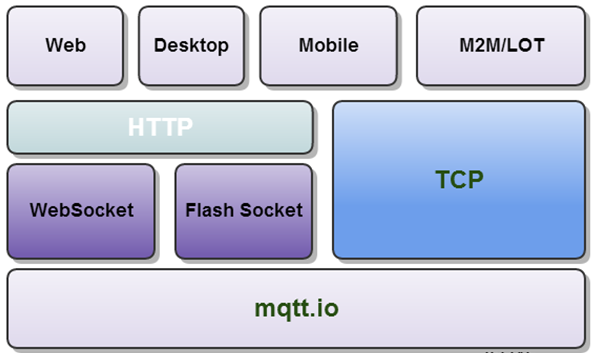
\includegraphics[width=.9\textwidth]{comunicacao.png}\footnotemark
	\end{figure}
	
	\footnotetext{http://images.cnitblog.com/blog/120296/201406/}
\end{frame}

%-------------------------------------------------
%% Controle:
%-------------------------------------------------
\subsection*{Controle}
\begin{frame}{Como controlar a aplicação?}
	\begin{itemize}
		\item A qualquer hora;
		\item De qualquer lugar.
	\end{itemize}
	
		\begin{figure}[H]
			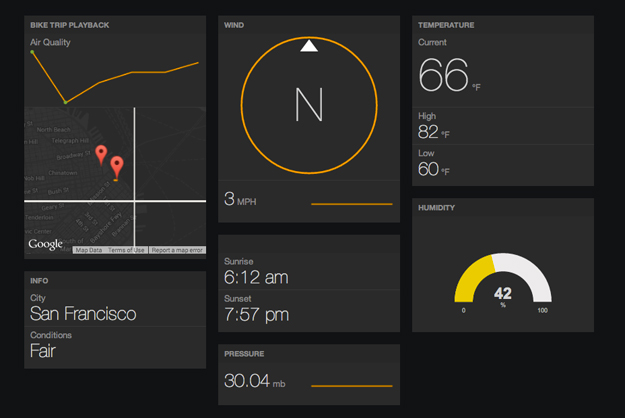
\includegraphics[width=.6\textwidth]{controle.jpg}\footnotemark
		\end{figure}
		
		\footnotetext{https://cdn.psfk.com/wp-content/uploads/2014/05/}
\end{frame}

%-------------------------------------------------
%% Estrutura:
%-------------------------------------------------
\section{Estrutura}
\label{sec:estrutura}

\subsection*{Integração}
\begin{frame}{Multidisciplinariedade}
	\begin{columns}
		\column{0.3\linewidth}
		\begin{itemize}
			\item Eletrônica;
			\item Robótica;
			\item Mecânica;
			\item Computação.
		\end{itemize}
		
		\column{0.7\linewidth}
		\begin{figure}[H]
			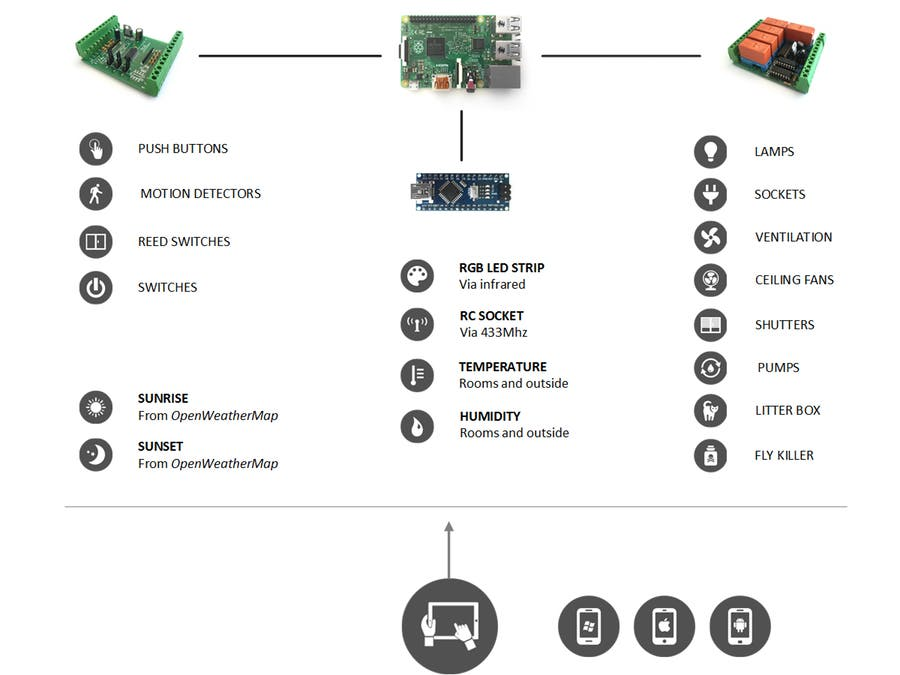
\includegraphics[width=1\textwidth]{multi.jpg}\footnotemark
		\end{figure}
	\end{columns}
	\footnotetext{https://hackster.imgix.net/uploads/cover\_image/file/81451/}
\end{frame}

%-------------------------------------------------
%% Hardware:
%-------------------------------------------------
\subsection*{Hardware}
\begin{frame}{Raspberry Pi}
	\begin{figure}[H]
		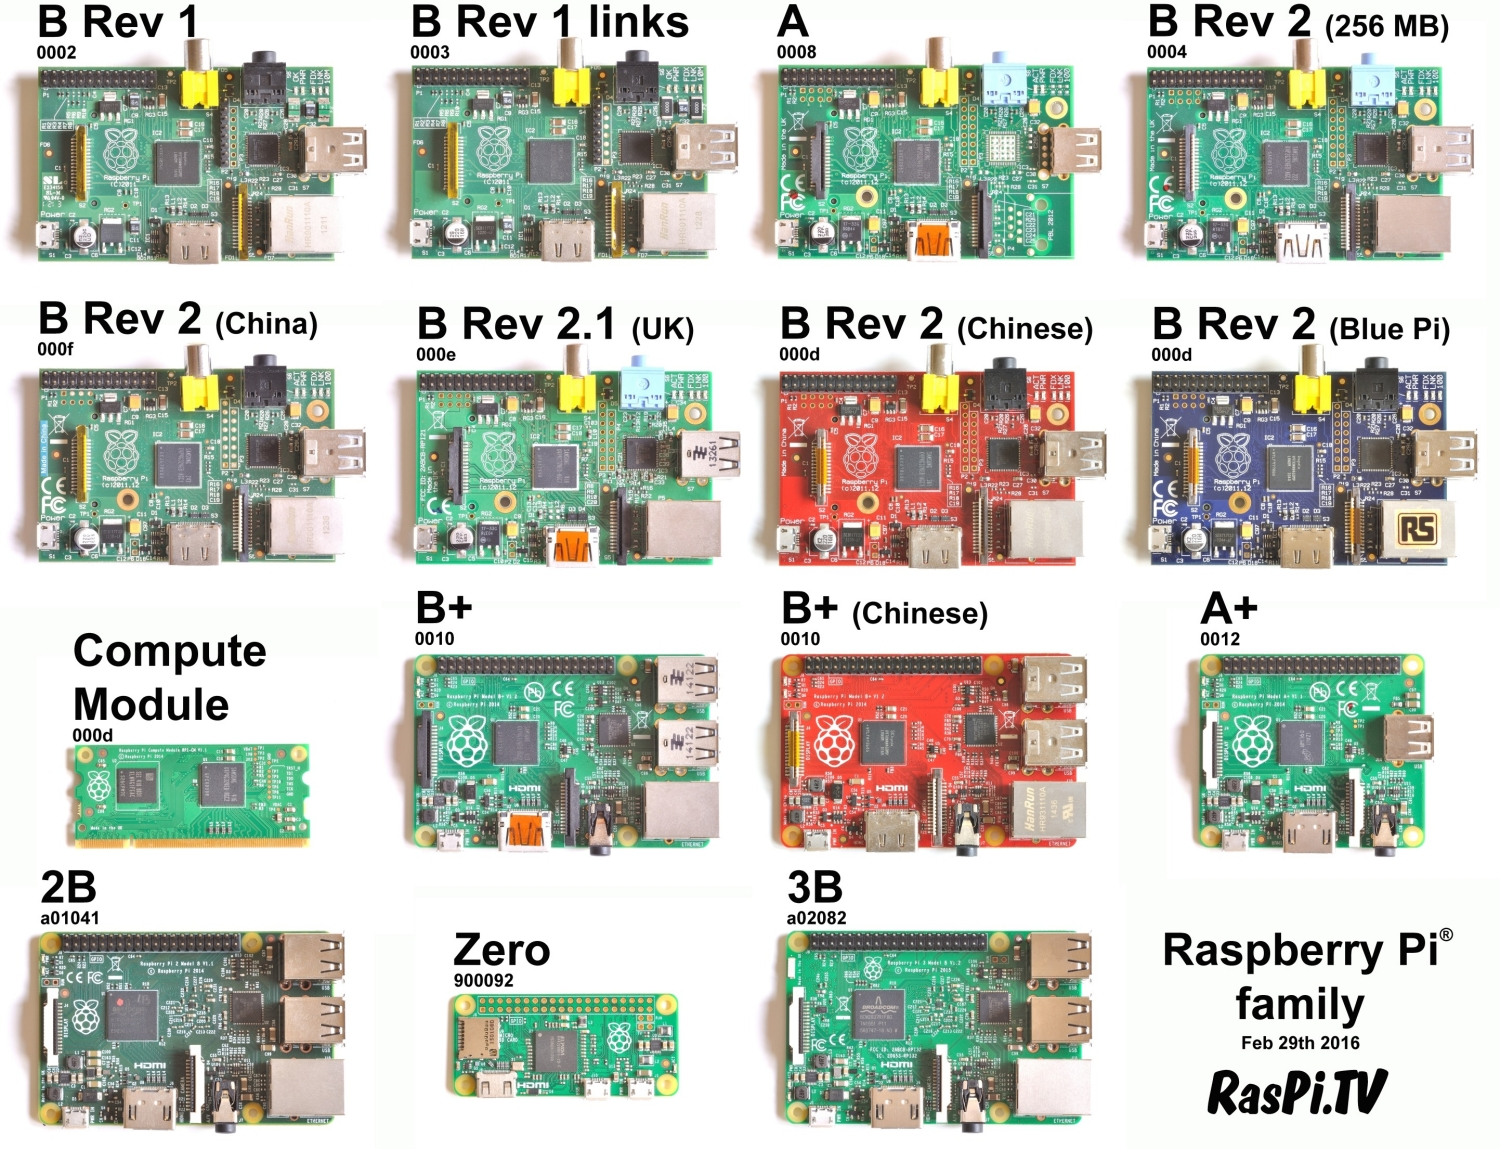
\includegraphics[width=.7\textwidth]{raspberryfamily.jpg}\footnotemark
	\end{figure}
	
	\footnotetext{http://raspi.tv/2016/raspberry-pi-family-photo-updated-to-include-pi3b-29-feb-2016}
\end{frame}

\begin{frame}{Arduino}
	\begin{figure}[H]
		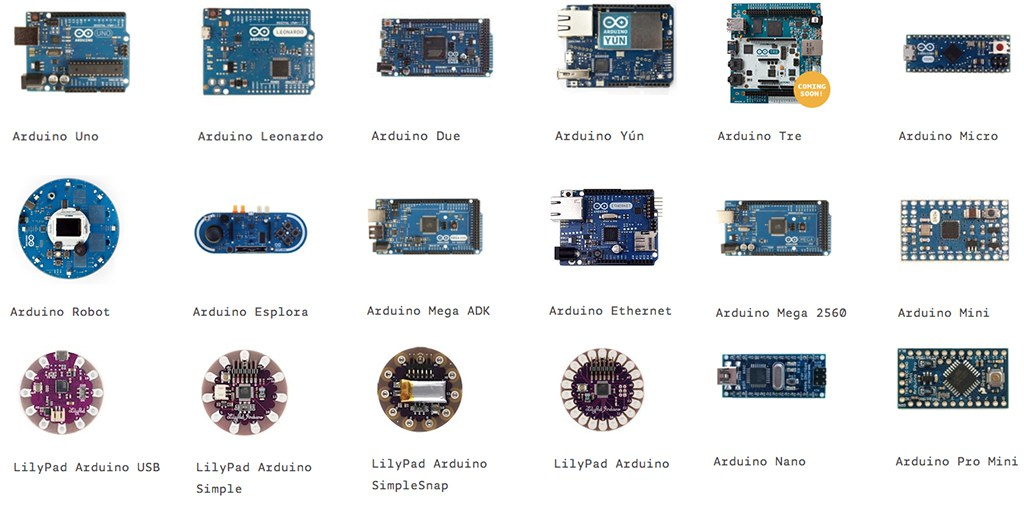
\includegraphics[width=1\textwidth]{arduinofamily.jpg}\footnotemark
	\end{figure}
	
	\footnotetext{https://i1.wp.com/electronicshacking.com/wp-content/uploads/2016/05/}
\end{frame}

\begin{frame}{ESP8266}
	\begin{figure}[H]
		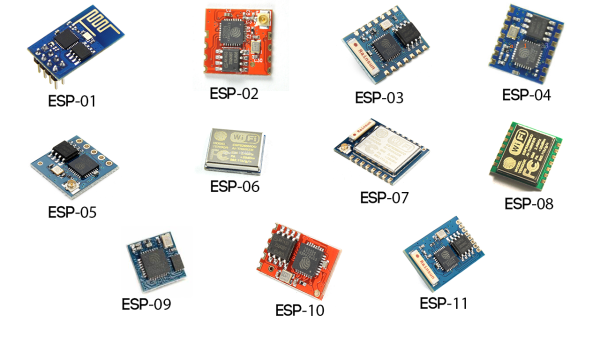
\includegraphics[width=.9\textwidth]{espfamily.png}\footnotemark
	\end{figure}
	
	\footnotetext{https://qph.ec.quoracdn.net/main-qimg-722e4cace72b92ca0efce373866d08c2}
\end{frame}

\begin{frame}{Módulo Relé}
	\begin{figure}[H]
		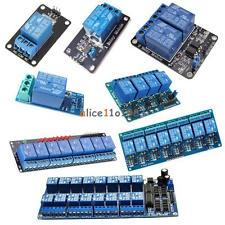
\includegraphics[width=.5\textwidth]{relayfamily.jpg}\footnotemark
	\end{figure}
	
	\footnotetext{http://thumbs.ebaystatic.com/images/m/mzkfWblEtqpHZfTceI9Bh9A/}
\end{frame}

%-------------------------------------------------
%% Software:
%-------------------------------------------------
\subsection*{Software}
\begin{frame}{}
	\begin{block}{Principais linguagens}
		\begin{itemize}
			\item Java;
			\item C/C++;
			\item Lua;
			\item Python;
			\item JavaScript;
			\item PHP.
		\end{itemize}
	\end{block}
\end{frame}

%-------------------------------------------------
%% Problemas:
%-------------------------------------------------
\section{Problemas}

\subsection*{Endereçamento}
\begin{frame}{}
	\begin{figure}[H]
		
\includegraphics[width=1\textwidth]{ipv4_stock.jpg}\footnotemark
	\end{figure}
	
	\footnotetext{https://victorh2007.files.wordpress.com/2014/06/}
\end{frame}

\subsection*{Segurança}
\begin{frame}{}
	\begin{block}{\cite{ComputerWorld}}
		\begin{itemize}
			\item Com tantas coisas conectadas à web, os institutos de pesquisa apontam aspectos negativos em relação à segurança. Eles indicam que dentro de \textbf{dois anos}, 90\% de todas as redes de TI terão uma falha de segurança derivada da IoT.
			\item Em 2013, hackers americanos invadiram um carro conectando-se à porta serial do veículo. Esse tipo de conexão é comumente utilizada para análise e manutenção dos veículos.
			\item Em 2015, eles repetiram o ataque via \textit{wireless}.
		\end{itemize}
	\end{block}
\end{frame}

\subsection*{Privacidade}
\begin{frame}{}
	\begin{block}{\cite{PedroValente} e \cite{P2413}}
		\begin{itemize}
			\item Proteção de dados pessoais;
			\item Hábitos, localização, interesses e preferências pessoais;
			\item Fluxo constante de informação;
			\item Normalização dos sistemas inteligentes.
		\end{itemize}
	\end{block}
\end{frame}

%-------------------------------------------------
%% Como começar:
%-------------------------------------------------
\section{Por onde começar?}
\label{sec:comeco}

\subsection*{Pesquise}
\begin{frame}{}
	\begin{block}{\textit{Links} para leitura (nas referências)}
		\begin{itemize}
			\item Windows 10 IoT \cite{WindowsIot};
			\item Intel IoT \cite{IntelIot};
			\item Raspberry and Google IoT Project \cite{RaspberryGoogleIot};
			\item Arduino IoT \cite{ArduinoIot}.		
		\end{itemize}
	\end{block}
\end{frame}

\subsection*{Faça Você Mesmo!}
\begin{frame}{}
	\begin{block}{\textit{Links} para praticar (nas referências)}
		\textbf{Pré-requisito: Inglês básico}
		\begin{itemize}
			\item Dweet.io - A rede social das máquinas \cite{DweetIot};
			\item ThingSpeak - Análise de dados \cite{ThingSpeakIot};
			\item Highcharts - Análise de dados e gráficos \cite{HighChartsIot};
			\item FreeBoard - Controle das coisas \cite{FreeBoardIot};
			\item Instructables - Ideias pra replicar (Básico) \cite{InstructablesIot}. 
			\item Hackaday - Ideias pra replicar (Avançado) \cite{HackadayIot}.
		\end{itemize}
	\end{block}
	\begin{figure}[H]
		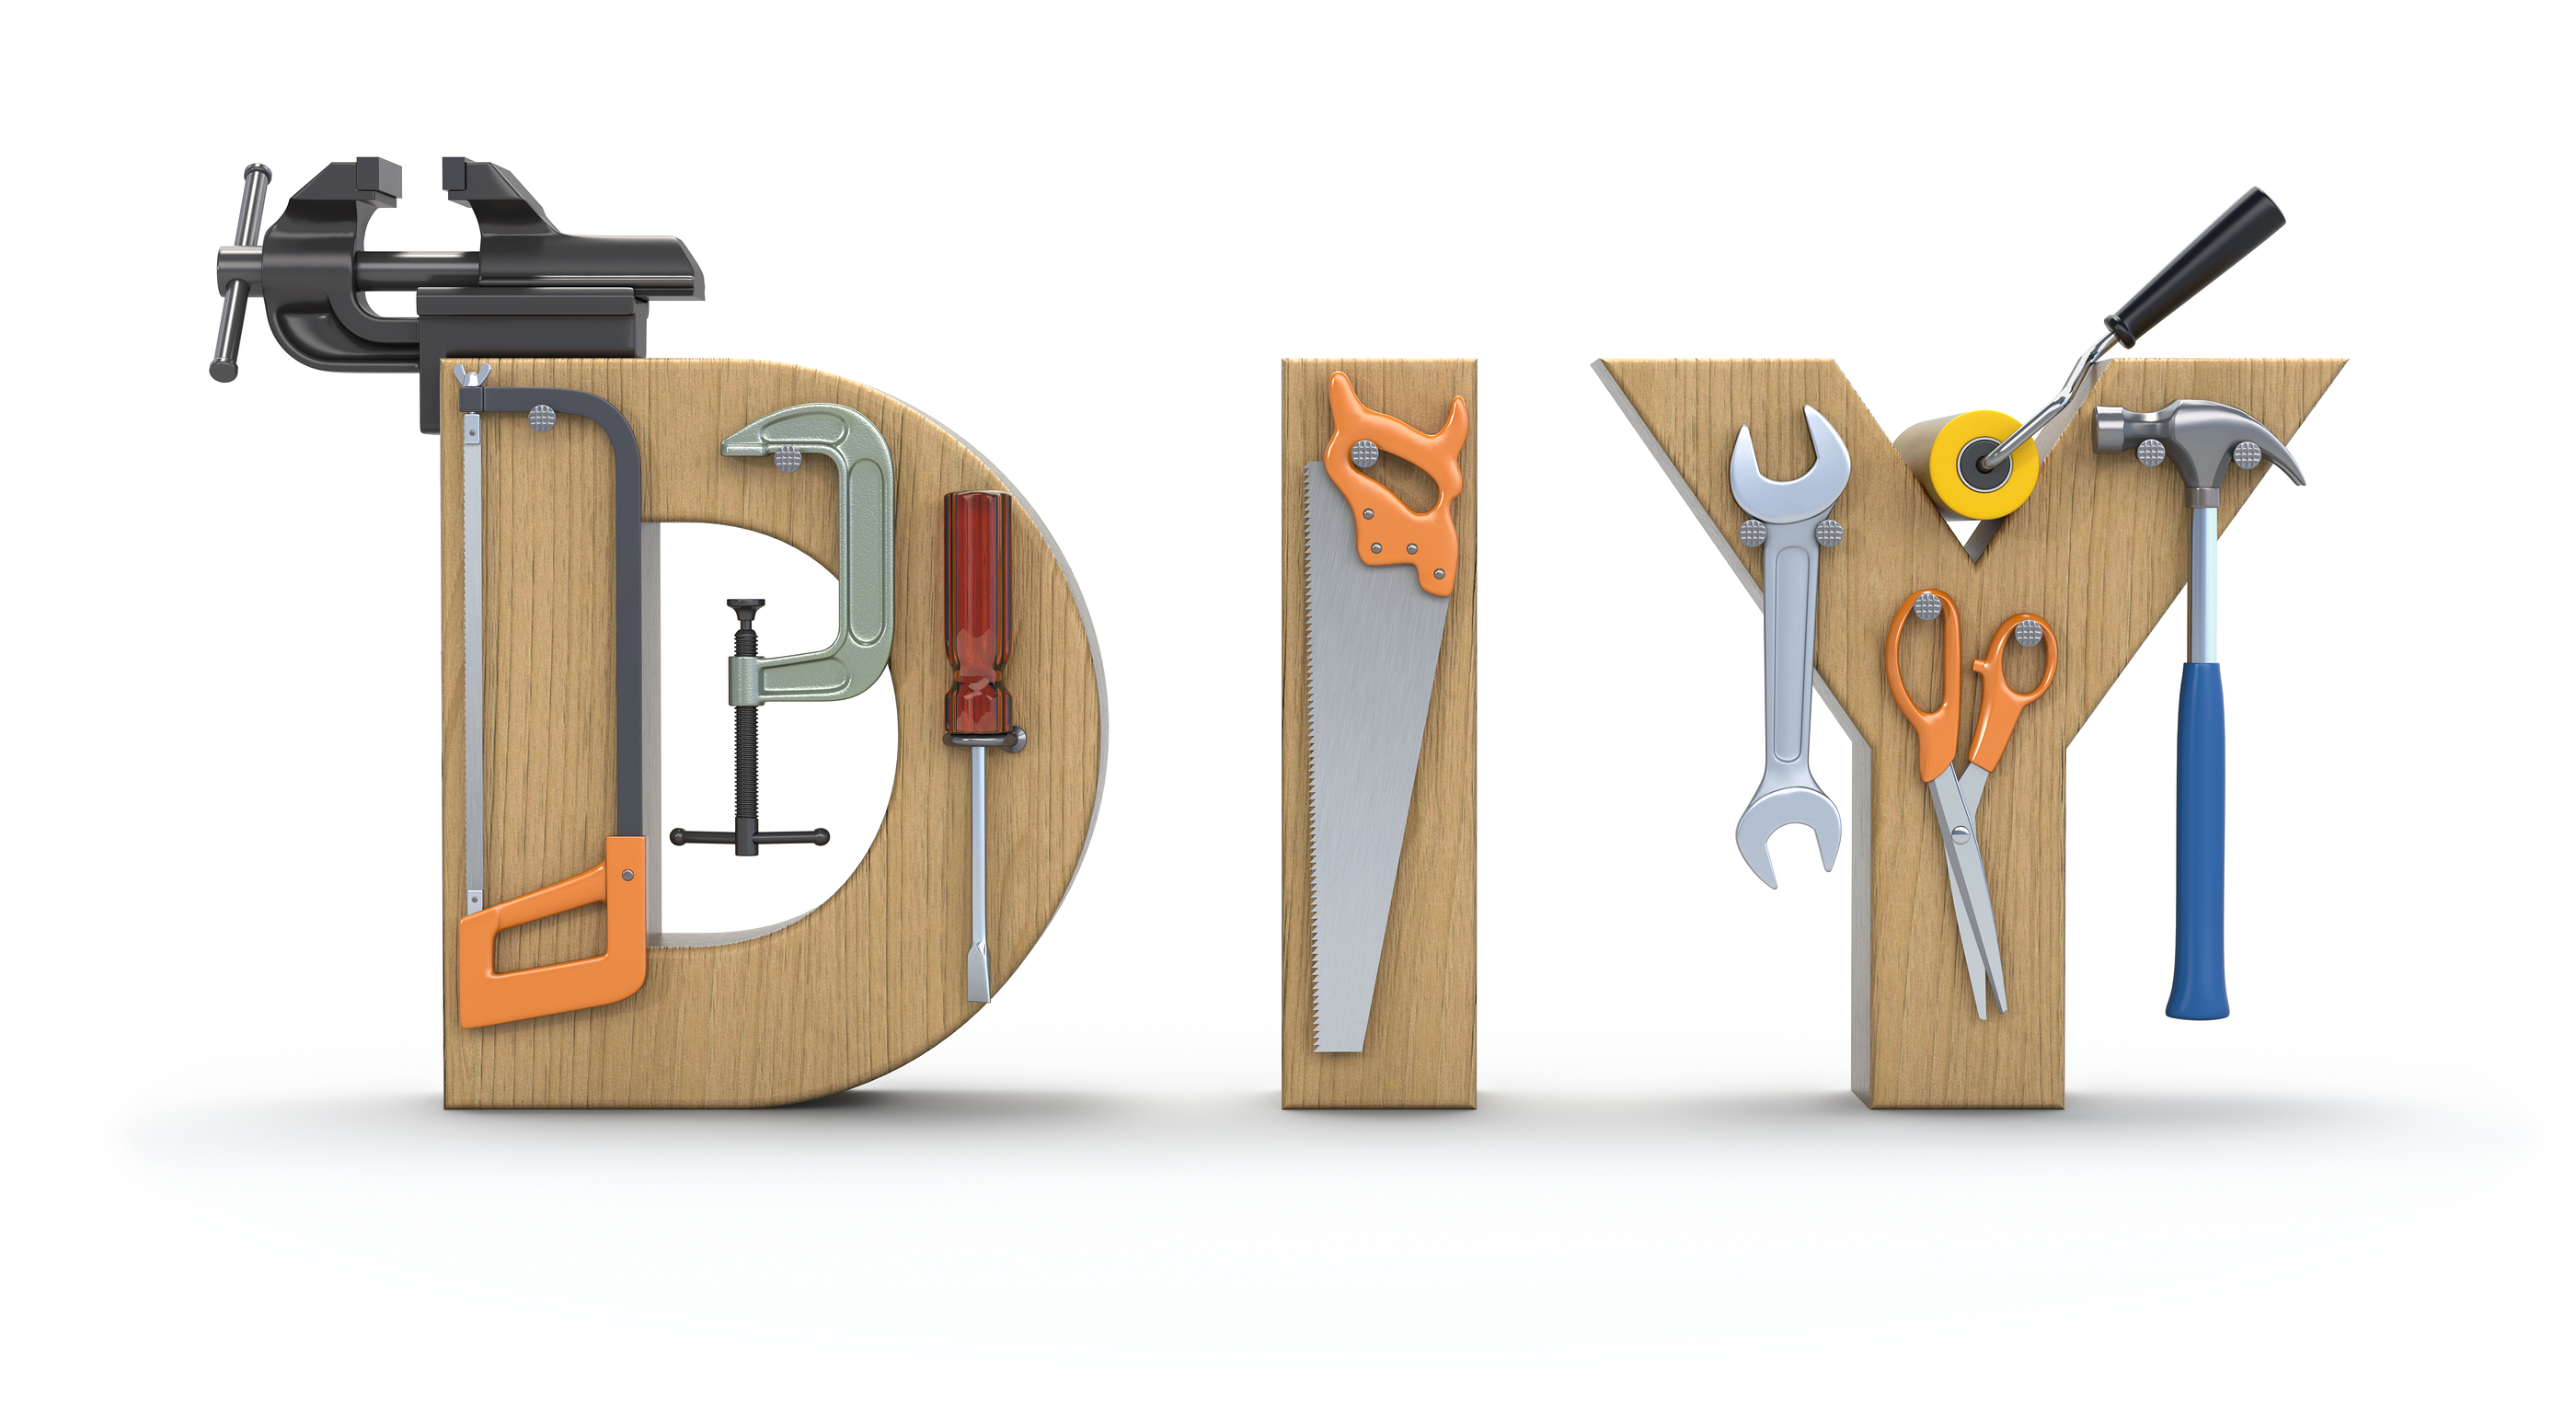
\includegraphics[width=.5\textwidth]{diy.jpg}\footnotemark
	\end{figure}
	
	\footnotetext{http://mydogsjournal.com/wp-content/uploads/2013/12/}
\end{frame}
	%\include{recapitulacao}
	
	% Elementos pós textuais
	\section*{Referências}
\begin{frame}[allowframebreaks, t]{\insertsection}	
	\bibliographystyle{apalike} %unsrt, plain, abbrv, apa
	\footnotesize \bibliography{refs}
\end{frame}
	\section*{Obrigado!}
\label{sec:obrigado}

\subsection*{Dúvidas? Entre em Contato!}
\begin{frame}
	\begin{block}{}
		\begin{center}
			\textbf{\mysubject}: \\[2ex] \mytitle\\[1ex]
		\end{center}
	\end{block}
	
	\vspace{1ex}
	
	\begin{center}
		\myauthor \\[4ex]          	
		 
\includegraphics[height=.5cm,keepaspectratio]{mail.png}\textcolor{white}{-} \myauthoremail \\
		 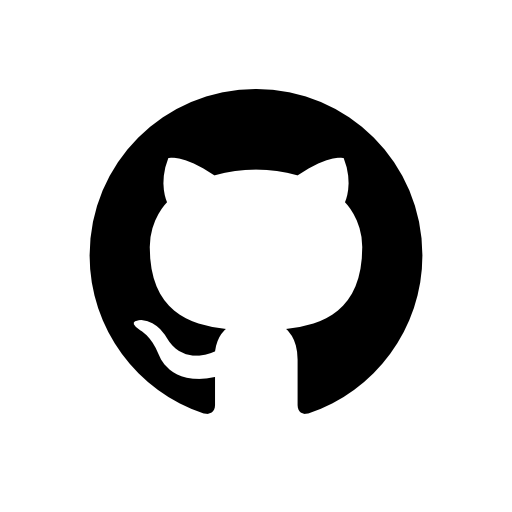
\includegraphics[height=.7cm,keepaspectratio]{github.png}\textcolor{white}{-}\myauthorgit \\[4ex]
	\end{center}	
	
	\begin{columns}[T]
		\begin{column}[T]{2cm}		
			
\includegraphics[height=1.0cm,keepaspectratio]{doctum.png}\centering
		\end{column}
		
		\begin{column}[T]{2cm}		
			
\includegraphics[height=1.0cm,keepaspectratio]{fic.png}\centering
		\end{column}
		
		\begin{column}[T]{2cm}		
			
\includegraphics[height=1.0cm,keepaspectratio]{ime.jpg}\centering
		\end{column}
		
		\begin{column}[T]{2cm}	
			
\includegraphics[height=1.0cm,keepaspectratio]{lab.png}\centering	
		\end{column}
	\end{columns}
	
	\vspace{3ex}
\end{frame}
\end{document}